Ben Trout

2014-10-24

CAD Designing, Field Assembly

\begin{tabular}{|p{5cm}|p{5cm}|}
\hline
CAD Designing&
Our current plan for launching the balls into the tubes is a slingshot. But we need a ball holder that will hold the balls and release them into the tub. The best way to do this is to make a piece on CREO that can perfectly fit a ball and has four holes that can attach to the surgical tubing. Me and Filip will were in charge of building this piece on CREO.
\\
\hline
Field Assembly&
Now that I have all the pieces cut and ready to be assembled some members from other teams were willing to put it together. Rob, Eric, and JJ are going to put the pieces together. I got them started and went out to make sure their on the right path and putting all the pieces together correctly. I plan on helping them less and less.
\\
\hline
\end{tabular}

\section*{CAD Designing}
I was in charge of designing the ball holder for our slingshot and building it on Creo. It was pretty hard as I'm new to Creo and it will take me a while to get used to. Will Werst, a member on my FRC team, helped me make the piece on Creo. He's a great teacher who knows a lot about Creo. With his guidance I was able to build the part using the revolve tool. Now all we have to do is take this piece that I CAD'd up and bring it to FRC. They have a 3D printer that can print our piece for us. CADing up pieces can be incredibly useful. If we need to make a slight change to the design because the ball wouldn't fit in the cup we can easily just make the changes in CREO and spit out the piece again on the 3D printer. Now that I know the basics of CREO, me and Filip plan on designing our entire robot on CREO and this is what we'll be working on next week.

\section*{Field Assembly}
It was a rough start for the build team but they’ve got it all figured out now. It took them a couple days to figure out how to put it together, but they have all the holes for one ramp predrilled and will start putting it together next week. I’ll let them off on their on and we should have a built field here soon. 

\begin{center}
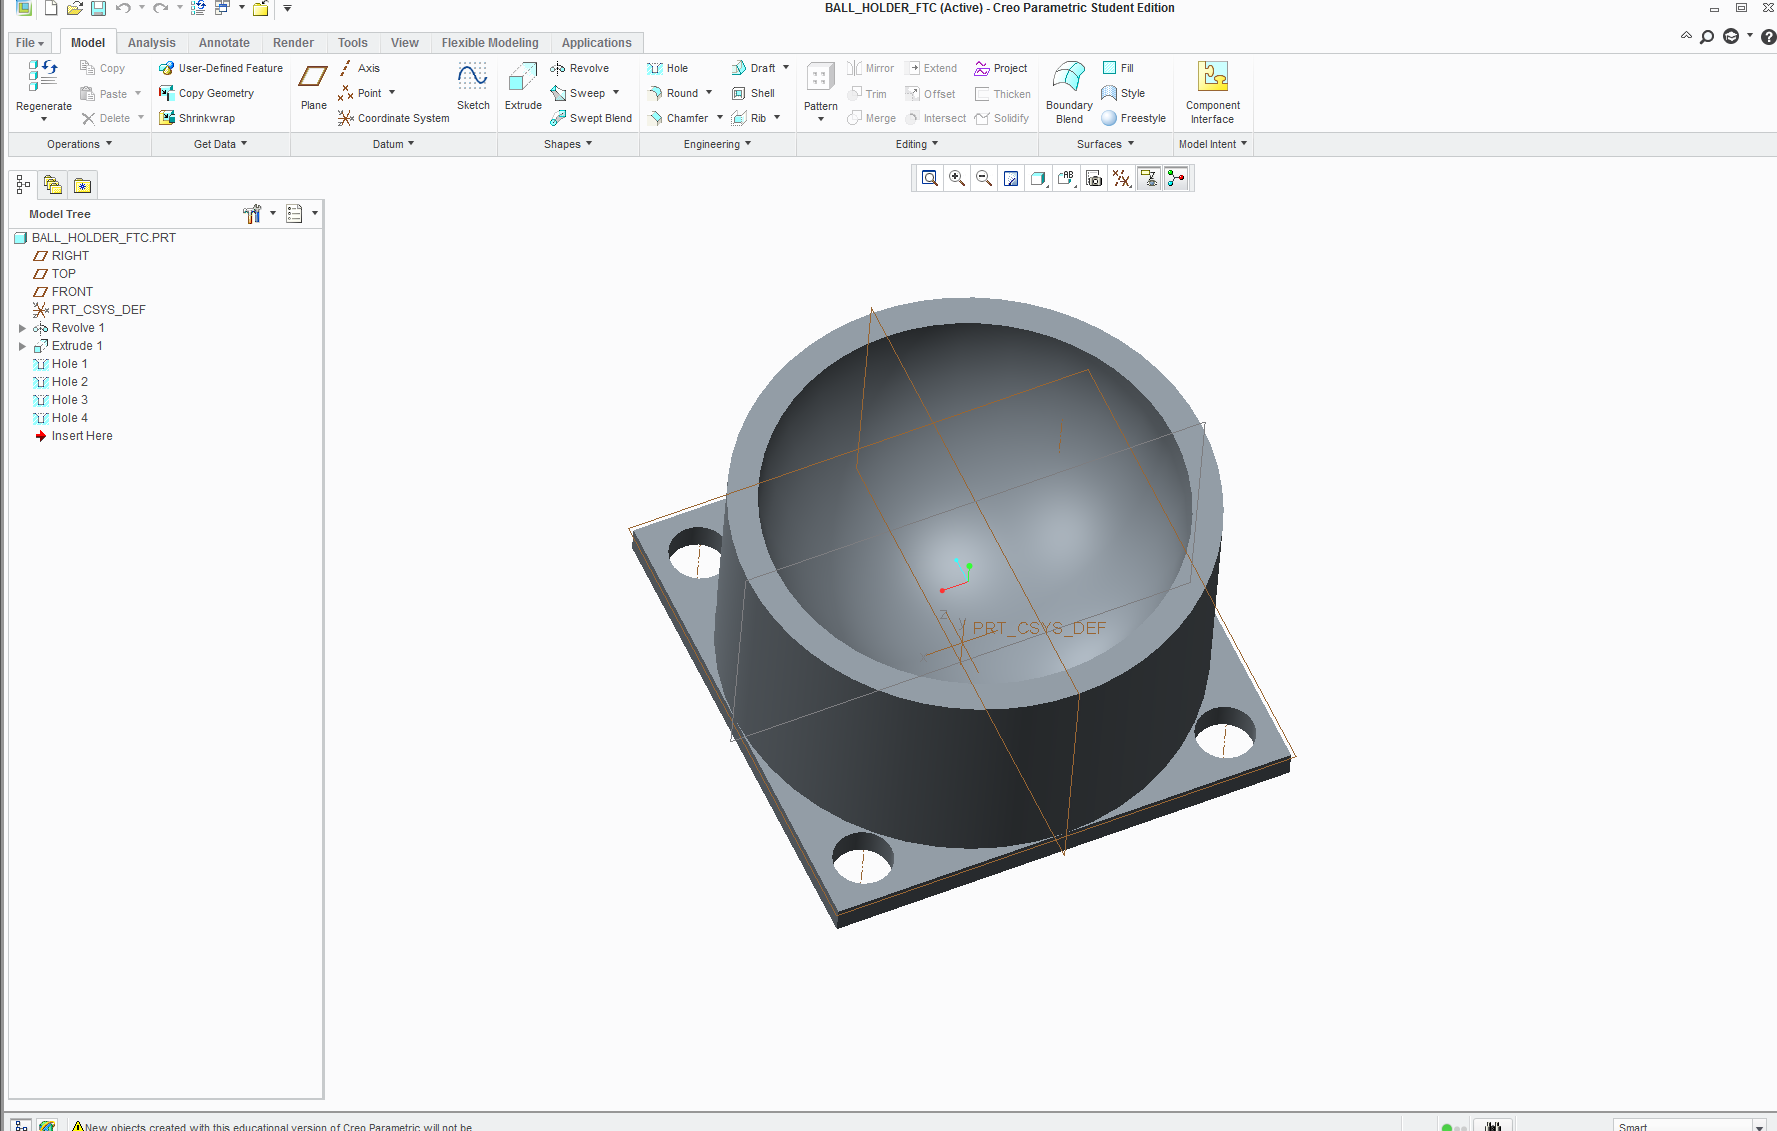
\includegraphics[width=10cm]{./Entries/Images/BallHolder.PNG}
\end{center}

CAD image of ball holder
